% -----------------------------------------------------------
% 4.3 การออกแบบระบบการเล่น
% -----------------------------------------------------------
\section{การออกแบบระบบการเล่น}

\subsection{วิธีการเล่นเกม (How to Play)}

ผู้เล่นรับบทเป็นกัปตันเรือขนส่งสินค้า มีหน้าที่สั่งการลูกเรือเพื่อนำเรือไปเทียบท่าปลายทางอย่างปลอดภัย กติกาการเล่นหลักมีดังนี้

\begin{enumerate}[label=\arabic*)]
    \item \textbf{การควบคุมผ่านวิทยุ:} ผู้เล่นไม่มีปุ่มบังคับหางเสือหรือเครื่องยนต์โดยตรง แต่ต้องออกคำสั่งเป็นภาษาอังกฤษทางวิทยุถึงลูกเรือปัญญาประดิษฐ์ ด้วยเสียง (ปุ่ม T) หรือพิมพ์คำสั่ง (ปุ่ม Enter) ขั้นตอนการสั่งการโดยละเอียดแสดงในตารางที่ \ref{tab:uc_order}
    \item \textbf{การหลบหลีกสิ่งกีดขวาง:} ร่องน้ำมีชายฝั่งและแนวหินกั้นทั้งสองข้าง และมีหิน แนวหินโสโครก สันดอน และทุ่นระเบิดกระจายอยู่ภายในร่องน้ำ ทุ่นระเบิดมีตั้งแต่ระดับ Normal ขึ้นไป และการชนทุ่นระเบิดทำให้เสียตู้สินค้า 2 ตู้ ส่วนสันดอนทำให้เรือเกยตื้นโดยไม่เสียหาย และผู้เล่นต้องสั่งถอยเรือออก ผู้เล่นต้องประเมินสถานการณ์จากภาพมุมไอโซเมตริกและเรดาร์ แล้วออกคำสั่งให้ทันเวลา เช่น ``Starboard fifteen'' หรือ ``Stop engine''
    \item \textbf{การตอบสนองของลูกเรือ:} หากลูกเรือเข้าใจคำสั่ง ลูกเรือที่รับผิดชอบจะทวนคำสั่งและบังคับเรือ ซึ่งเคลื่อนที่ตามแบบจำลองที่มีแรงเฉื่อย หากไม่เข้าใจ ลูกเรือจะตอบกลับตามบริบทหรือขอให้พูดซ้ำ (Say again)
    \item \textbf{ผลลัพธ์ของภารกิจ:}
    \begin{itemize}[leftmargin=1.5em,labelindent=0pt]
        \item \textbf{สำเร็จ (Cargo Delivered):} นำเรือถึงท่าปลายทาง ขอเทียบท่า (Request Docking) และผูกเรือ (Make Fast) ได้ก่อนความทนทานของตัวเรือหมด โดยการชนแต่ละครั้งทำให้ตู้สินค้าตกน้ำและค่าตอบแทนลดลง
        \item \textbf{ล้มเหลว (Ship Lost):} ชนสิ่งกีดขวางจนความทนทานของตัวเรือเหลือศูนย์ เรือลากจูงจะลากเรือกลับท่าโดยผู้เล่นเสียค่าลากเรือ
    \end{itemize}
\end{enumerate}

\subsection{กระบวนการเล่นหลัก (Core Game Loop)}

กระบวนการเล่นหลักแสดงกิจกรรมที่ผู้เล่นทำซ้ำระหว่างการเดินเรือหนึ่งรอบ และการโต้ตอบระหว่างผู้เล่น ลูกเรือ และแบบจำลองการเคลื่อนที่ของเรือ ดังภาพที่ \ref{fig:gameloop} ส่วนการเปลี่ยนสถานะของระบบทั้งเกม ตั้งแต่เมนูหลักจนถึงหน้าสรุปผล แสดงแยกเป็นแผนภาพสถานะในภาพที่ \ref{fig:state_main} ในภาคผนวก ค

\MermaidAdjustBoxOpts{max width=\linewidth, max height=0.88\textheight, center}
\begin{figure}[!htbp]
\centering
\begin{mermaid}
%%{init: {'flowchart': {'nodeSpacing': 25, 'rankSpacing': 28}}}%%
graph TD
    A[เริ่มภารกิจ] --> B[ประเมินสถานการณ์จากเรดาร์และภาพทะเล]
    B --> E[ผู้เล่นออกคำสั่ง เสียงหรือพิมพ์]
    E --> F[แปลงเสียงเป็นข้อความ]
    F --> G{ตัวแยกคำสั่งพบคำสั่งหรือไม่}
    G -- ไม่พบ --> Q[GPT-4o mini จำแนกเจตนา]
    Q --> R{พบคำสั่งหรือไม่}
    R -- ไม่พบ --> H[ลูกเรือสนทนาตอบ หรือขอให้พูดซ้ำ]
    H --> B
    R -- พบ --> I[ลูกเรือทวนคำสั่ง]
    G -- พบ --> I
    I --> J[เรือเคลื่อนที่ตามคำสั่ง]
    J --> K{ชนสิ่งกีดขวางหรือไม่}
    K -- ชน --> N[ความทนทานของตัวเรือลดลง ตู้สินค้าตกน้ำ]
    N --> O{ความทนทานเหลือ 0 หรือไม่}
    O -- เหลือ 0 --> P[Ship Lost ลากเรือกลับท่า]
    O -- ยังไม่เหลือ 0 --> B
    K -- ไม่ชน --> L{ถึงท่าปลายทางหรือยัง}
    L -- ยังไม่ถึง --> B
    L -- ถึงแล้ว --> S[ขอเทียบท่าและผูกเรือ]
    S --> M[Cargo Delivered]
\end{mermaid}
\caption{แผนภาพกระบวนการเล่นหลัก (Core Game Loop)}
\label{fig:gameloop}
\end{figure}
\MermaidAdjustBoxOpts{max width=\linewidth, max height=0.65\textheight, center}

จากภาพที่ \ref{fig:gameloop} ผู้เล่นออกคำสั่งได้ตลอดการเดินเรือ ไม่เฉพาะเมื่อพบสิ่งกีดขวาง ความท้าทายหลักของเกมไม่ได้อยู่ที่การกดปุ่ม แต่อยู่ที่การบริหารเวลาในการพูดคำสั่งและการแก้ปัญหาการสื่อสาร ขณะที่เรือยังคงเคลื่อนที่ต่อเนื่อง

\subsection{สถาปัตยกรรมของระบบ (System Architecture)}

สถาปัตยกรรมระบบเกมเดินเรือด้วยระบบสั่งการด้วยเสียงแสดงดังภาพที่ \ref{fig:architecture}

\begin{figure}[!htbp]
\centering
\begin{mermaid}
graph TD
    subgraph Client["Player PC (Client)"]
        Unity["Unity Engine (Game Client)"]
        Mic["Microphone (Audio Input)"]
        Speaker["Speaker/Headphones (Audio Output)"]
    end

    subgraph Core["Core Systems"]
        GameLogic["C# Game Logic, Command Parser and Ship Physics"]
        UI["UI and HUD"]
        STT["Speech-to-Text (Whisper, whisper.cpp on-device)"]
        TTS["Windows Speech (TTS)"]
    end

    subgraph ExternalAPI["External API"]
        LLM["OpenAI API (GPT-4o mini)"]
    end

    Mic -->|Voice Input| Unity
    Unity -->|Audio Clip| STT
    STT -->|Text| GameLogic
    GameLogic -->|unclear text / chat only| LLM
    LLM -->|intent JSON / reply text| GameLogic
    GameLogic -->|Control| UI
    GameLogic -->|crew line text| TTS
    TTS -->|crew voice| Speaker
\end{mermaid}
\caption{สถาปัตยกรรมของระบบเกม}
\label{fig:architecture}
\end{figure}

จากภาพที่ \ref{fig:architecture} ระบบทำงานบนเกมเอนจิน Unity เป็นหลัก โดยรับเสียงพูดภาษาอังกฤษผ่านไมโครโฟน และแปลงเป็นข้อความด้วยโมเดลการรู้จำเสียง Whisper~\cite{radford2023} ซึ่งทำงานภายในเครื่องของผู้เล่นผ่านไลบรารี whisper.cpp โดยไม่ส่งเสียงออกไปยังเครือข่าย จากนั้นตัวแยกคำสั่งภายในเครื่องแปลข้อความเป็นคำสั่งควบคุมเรือ ระบบส่งข้อความไปยัง GPT-4o mini ผ่านเครือข่ายเฉพาะ 2 กรณี ได้แก่ คำสั่งที่ตัวแยกคำสั่งไม่เข้าใจ (เพื่อจำแนกเจตนาเป็น JSON) และการสนทนากับลูกเรือ (เพื่อสร้างข้อความตอบกลับ) GPT-4o mini ส่งกลับมาเพียงข้อความ ส่วนเสียงของลูกเรือสร้างด้วยระบบสังเคราะห์เสียงของ Windows (Windows Speech) บนเครื่องของผู้เล่น

\subsection{แผนภาพการติดตั้ง (Deployment Diagram)}

แผนภาพการติดตั้งแสดงการจัดวางส่วนประกอบของเกมบนเครื่องของผู้เล่น ดังภาพที่ \ref{fig:deployment} เกมทั้งหมดรวมถึงโมเดลการรู้จำเสียงติดตั้งอยู่ในเครื่องคอมพิวเตอร์ของผู้เล่น มีเพียงบริการ OpenAI ที่เรียกผ่านอินเทอร์เน็ต

\begin{figure}[!htbp]
\centering
\begin{mermaid}
graph TD
    subgraph PC["เครื่องคอมพิวเตอร์ของผู้เล่น (Windows 10/11)"]
        Mic["ไมโครโฟน / ชุดหูฟัง"]
        subgraph App["SpeechCruiser.exe (Unity)"]
            Game["ตรรกะเกม ฟิสิกส์เรือ และ UI"]
            Whisper["whisper.cpp + ggml-base.en.bin"]
            TTS["เสียงลูกเรือ (Windows Speech)"]
        end
        Prefs["PlayerPrefs (Registry)"]
        Logs["แฟ้ม CSV ในโฟลเดอร์ Sessions"]
        Key["OPENAI_API_KEY หรือ openai.key"]
    end

    subgraph Cloud["บริการภายนอก"]
        OpenAI["OpenAI API (GPT-4o mini)"]
    end

    Mic -- "เสียงพูด" --> Whisper
    Whisper -- "ข้อความ" --> Game
    Game --> TTS
    Game --> Prefs
    Game --> Logs
    Key -.-> Game
    Game -- "HTTPS :443 (เฉพาะเมื่อจำเป็น)" --> OpenAI
\end{mermaid}
\caption{แผนภาพการติดตั้งระบบ}
\label{fig:deployment}
\end{figure}

จากภาพที่ \ref{fig:deployment} ระบบไม่ส่งเสียงของผู้เล่นออกนอกเครื่อง ข้อมูลที่ส่งไปยังบริการ OpenAI มีเพียงข้อความที่ถอดได้และสถานะของเรือ

\subsection{โครงสร้างโฟลเดอร์ของโครงการ (Project Structure)}

โครงสร้างแฟ้มข้อมูลของโครงการที่พัฒนาด้วยเกมเอนจิน Unity แสดงดังตารางที่ \ref{tab:folder}

\begin{table}[!htbp]
\centering
\caption{โครงสร้างโฟลเดอร์หลักของโครงการ}
\label{tab:folder}
\begin{tabular}{|L{4.50cm}|L{9.20cm}|}
\hline
\textbf{โฟลเดอร์} & \textbf{คำอธิบาย} \\
\hline
\texttt{Assets/Scenes/} & ฉาก Menu (เมนูหลักและโหมดเนื้อเรื่อง) และฉาก Game (อู่ต่อเรือ การเดินเรือ และหน้าสรุปผล) \\ \hline
\texttt{Assets/Script/} & ชุดคำสั่งภาษา C\# สำหรับแบบจำลองการเคลื่อนที่ของเรือ การรับคำสั่งเสียง ลูกเรือ และระบบ UI โดยมีโฟลเดอร์ย่อย เช่น \texttt{Command/} (ตัวแยกคำสั่ง) \texttt{Ship/} (สร้างโมเดลเรือของผู้เล่นด้วยโค้ด) \texttt{Teaching/} (ระบบช่วยสอนภาษาและบันทึกผลการทดลอง) และ \texttt{Story/} (โหมดเนื้อเรื่อง) \\ \hline
\texttt{Assets/Script/LLMManager/} & ชุดคำสั่งสำหรับเชื่อมต่อ OpenAI API \\ \hline
\texttt{Assets/Whisper/} & แพ็กเกจ whisper.unity (ไลบรารี whisper.cpp) สำหรับรู้จำเสียงภายในเครื่อง โดยแฟ้มโมเดล ggml-base.en เก็บอยู่ที่ \texttt{Assets/StreamingAssets/Whisper/} \\ \hline
\texttt{Assets/Prefab/} & วัตถุสำเร็จรูป ได้แก่ ตู้สินค้า ทุ่นระเบิด แนวหิน และท่าเรือ \\ \hline
\texttt{Assets/Mesh/} & แฟ้มโมเดล 3 มิติ (3D Models) ของตู้สินค้า ทุ่นระเบิด แนวหิน และท่าเรือ \\ \hline
\texttt{Assets/Audio/} & ดนตรีประกอบและเสียงเอฟเฟกต์ (SFX) ส่วนเสียงทะเลและนกนางนวลสังเคราะห์ด้วยโค้ด \\ \hline
\texttt{Assets/UI/} & แฟ้มโครงหน้าจอ (UXML) และรูปแบบการแสดงผล (USS) ของ UI Toolkit สำหรับเมนู HUD และอู่ต่อเรือ \\
\hline
\end{tabular}
\end{table}

\subsection{การออกแบบหน้าจอ}

ผู้จัดทำออกแบบหน้าจอของเกมให้จำลองสถานการณ์การเดินเรือได้สมจริงและอ่านข้อมูลง่าย โดยไม่บดบังภาพทะเล หน้าจอหลักของเกมแสดงดังตารางที่ \ref{tab:mockups}

\begin{table}[!htbp]
\centering
\caption{รายการต้นแบบหน้าจอ}
\label{tab:mockups}
\begin{tabular}{|L{1.48cm}|L{3.44cm}|L{8.36cm}|}
\hline
\textbf{รหัสหน้าจอ} & \textbf{ชื่อหน้าจอ} & \textbf{ส่วนประกอบหลัก} \\
\hline
UI-01 & หน้าจอหลัก (Main Menu) & ชื่อเกม ปุ่มโหมดเนื้อเรื่อง (Story) ที่บอกภารกิจถัดไป ปุ่มเดินเรืออิสระ (Free Sail) ปุ่มเริ่มอาชีพใหม่ (New Career) ปุ่มตั้งค่า (Settings) ปุ่มออกเกม (Quit) และสถานะไมโครโฟนพร้อมคำแนะนำให้ทดสอบวิทยุ \\ \hline
UI-02 & หน้าจอเล่นเกม (Gameplay HUD) & ภาพเรือมุมไอโซเมตริก เรดาร์ เข็มทิศและองศาหัวเรือ คันโทรเลขเครื่องยนต์และความเร็ว ตัวแสดงมุมหางเสือ ความทนทานของตัวเรือ (Hull) กล่องสถานะวิทยุ ช่องวิทยุที่เลือก คำบรรยายบทพูดของลูกเรือ และคำแนะนำประโยคที่ควรพูด (Try Saying) \\ \hline
UI-03 & หน้าจออู่ต่อเรือ (Shipyard) & ยอดเงิน รายการงานขนส่งสินค้าตามระดับความยาก (Easy Normal Hard) พร้อมค่าตอบแทน ปุ่มอัปเกรดเรือ (Upgrade Ship) ซึ่งใช้เงินร่วมกับใบรับรองทักษะภาษา และปุ่มออกเรือ (Set Sail) โดยการซ่อมแซมเรือไม่มีค่าใช้จ่าย \\ \hline
UI-04 & หน้าจอสรุปผล (Result Screen) & หัวข้อ Cargo Delivered (Mission Complete ในโหมดเนื้อเรื่อง) หรือ Ship Lost ผลการเดินเรือ (ตู้สินค้าที่ส่งถึง หรือตู้สินค้าที่เสียและค่าลากเรือ จำนวนครั้งที่ชน เวลาที่ใช้) สรุปการสื่อสารทางวิทยุ (สัดส่วนคำสั่งที่ลูกเรือเข้าใจ จำนวนคำสั่งมาตรฐาน จำนวนครั้งที่ลูกเรือขอให้พูดซ้ำ เวลาเฉลี่ยในการสั่งหลังได้รับคำเตือน และจำนวนคำสั่งฉุกเฉินที่ทันเวลา) ความคืบหน้าของใบรับรอง เงินที่ได้รับ และคำแนะนำสำหรับรอบถัดไป \\ \hline
UI-05 & เมนูหยุดเกม (Pause) & ปุ่มเล่นต่อ (Resume) ตั้งค่า (Settings) เล่นบทฝึกสอนซ้ำ (Replay Tutorial) กลับเมนูหลัก (Main Menu) และออกเกม (Quit) \\ \hline
UI-06 & หน้าจอตั้งค่า (Settings) & เลือกไมโครโฟน ระดับเสียง ขนาดคำบรรยาย ปุ่มสั่งการและปุ่มสนทนา โหมดกดค้างหรือกดสลับเพื่อพูด และรหัสผู้เข้าร่วม (Participant Code) \\
\hline
\end{tabular}
\end{table}

\subsubsection{UI-01: หน้าจอหลัก (Main Menu)}

หน้าจอหลักเป็นหน้าแรกเมื่อเปิดเกม ใช้พื้นหลังสีกระดาษและภาพท่าเรือจริงจากในเกม ดังภาพที่ \ref{fig:ui_menu}

\begin{figure}[!htbp]
\centering
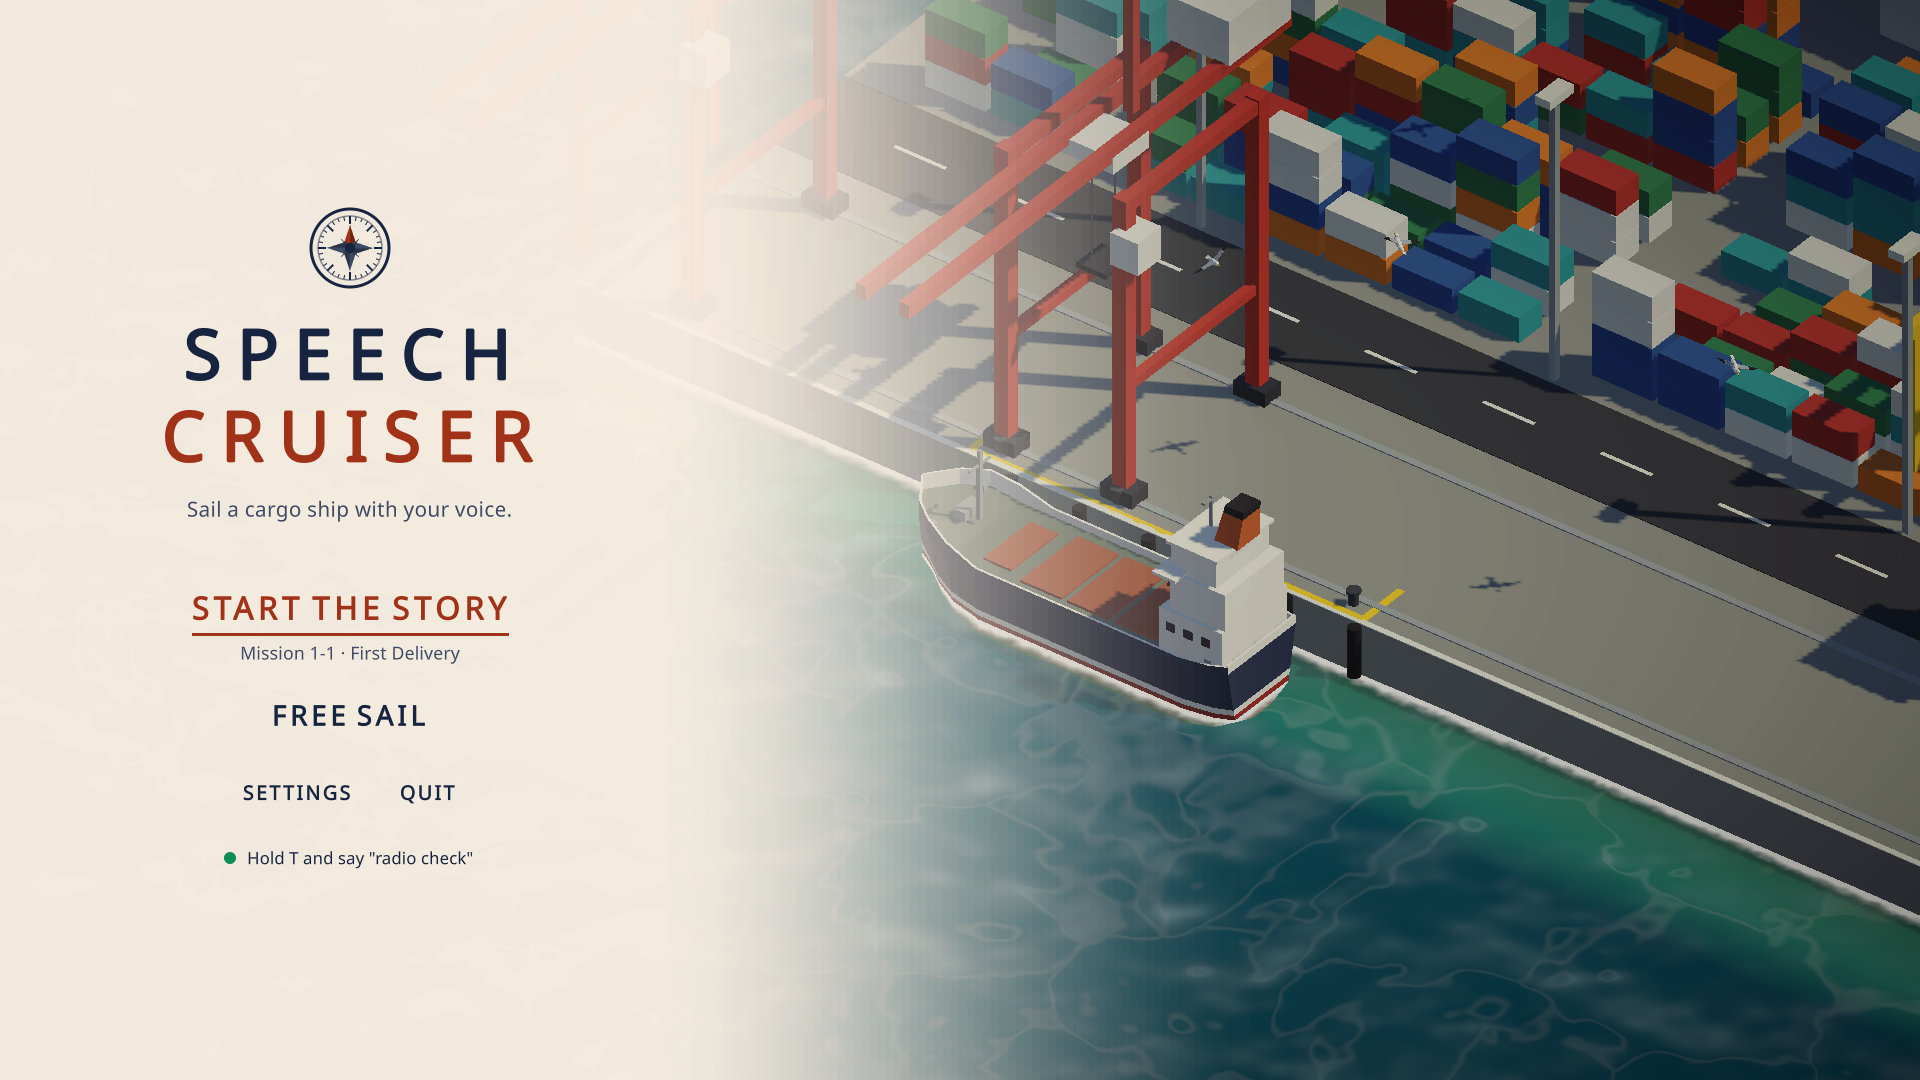
\includegraphics[width=0.8\textwidth]{Document/GameDev/images/MainMenu.png}
\caption{หน้าจอหลัก (UI-01)}
\label{fig:ui_menu}
\end{figure}

จากภาพที่ \ref{fig:ui_menu} ปุ่มโหมดเนื้อเรื่องแสดงชื่อภารกิจถัดไป (เช่น Mission 1-1 · First Delivery) ปุ่มเดินเรืออิสระพาไปยังอู่ต่อเรือ และด้านล่างแสดงสถานะไมโครโฟนพร้อมชวนให้ผู้เล่นทดสอบวิทยุด้วยคำว่า ``radio check'' ก่อนเริ่มเล่น

\subsubsection{UI-02: หน้าจอเล่นเกม (Gameplay HUD)}

หน้าจอเล่นเกมเป็นหน้าจอที่ผู้เล่นใช้ตลอดการเดินเรือ ออกแบบตามมุมมองไอโซเมตริก (Isometric View) เพื่อให้ข้อมูลที่จำเป็นครบถ้วนแต่ไม่บดบังภาพทะเล ดังภาพที่ \ref{fig:wf_gameplay}

\begin{figure}[!htbp]
\centering
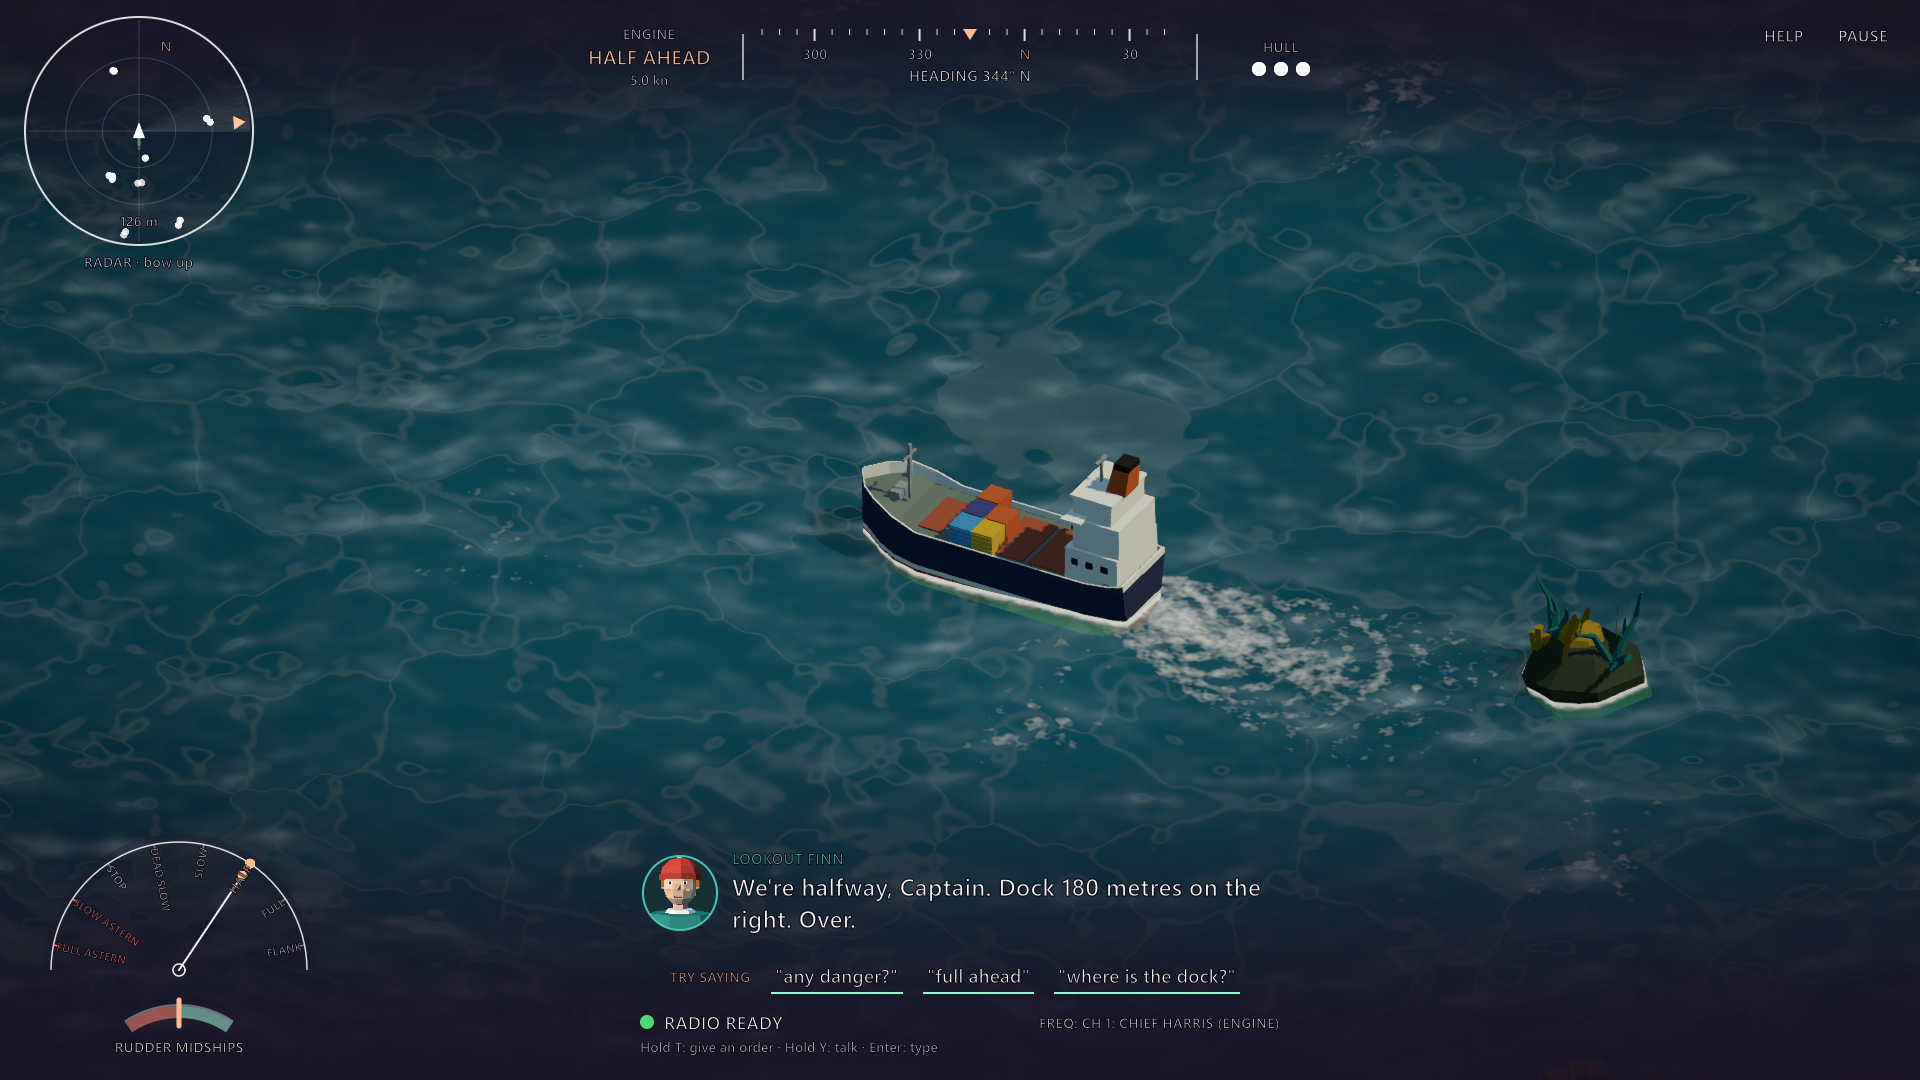
\includegraphics[width=0.8\textwidth]{Document/GameDev/images/StartUI.png}
\caption{หน้าจอเล่นเกม (UI-02)}
\label{fig:wf_gameplay}
\end{figure}

จากภาพที่ \ref{fig:wf_gameplay} ผู้เล่นมองเห็นตัวเรือ สภาพแวดล้อมทางทะเล และตำแหน่งของสิ่งกีดขวางโดยรอบจากมุมมองไอโซเมตริก องค์ประกอบบนหน้าจอมีดังนี้
\begin{itemize}
    \item แถบด้านบนกลางแสดงคำสั่งเครื่องยนต์และความเร็ว แถบเข็มทิศบอกองศาหัวเรือ และความทนทานของตัวเรือเป็นจุดกลมเรียงกัน (HULL) ซึ่งลดลงหนึ่งจุดเมื่อชน
    \item มุมซ้ายบนเป็นเรดาร์ที่แสดงร่องน้ำ แนวหิน ทุ่นระเบิด และท่าปลายทาง เพื่อช่วยประเมินสถานการณ์ล่วงหน้า
    \item มุมซ้ายล่างเป็นคันโทรเลขเครื่องยนต์ (Engine Telegraph) และตัวแสดงมุมหางเสือ (Rudder Angle Indicator)
    \item ด้านล่างกลางมีคำแนะนำประโยคที่ควรพูด (Try Saying) คำบรรยายบทพูดของลูกเรือ และกล่องวิทยุแสดงสถานะขณะรับเสียง (SENDING ORDER) และขณะแปลงเสียง (DECODING...)
\end{itemize}
กล่องวิทยุช่วยให้ผู้เล่นรู้ว่าควรเริ่มพูดหรือรอเมื่อใด จึงบริหารเวลาในการสื่อสารได้

\subsubsection{UI-03: หน้าจออู่ต่อเรือ (Shipyard)}

หน้าจออู่ต่อเรือเป็นจุดเริ่มของการเดินเรือแต่ละรอบ ดังภาพที่ \ref{fig:ui_shipyard}

\begin{figure}[!htbp]
\centering
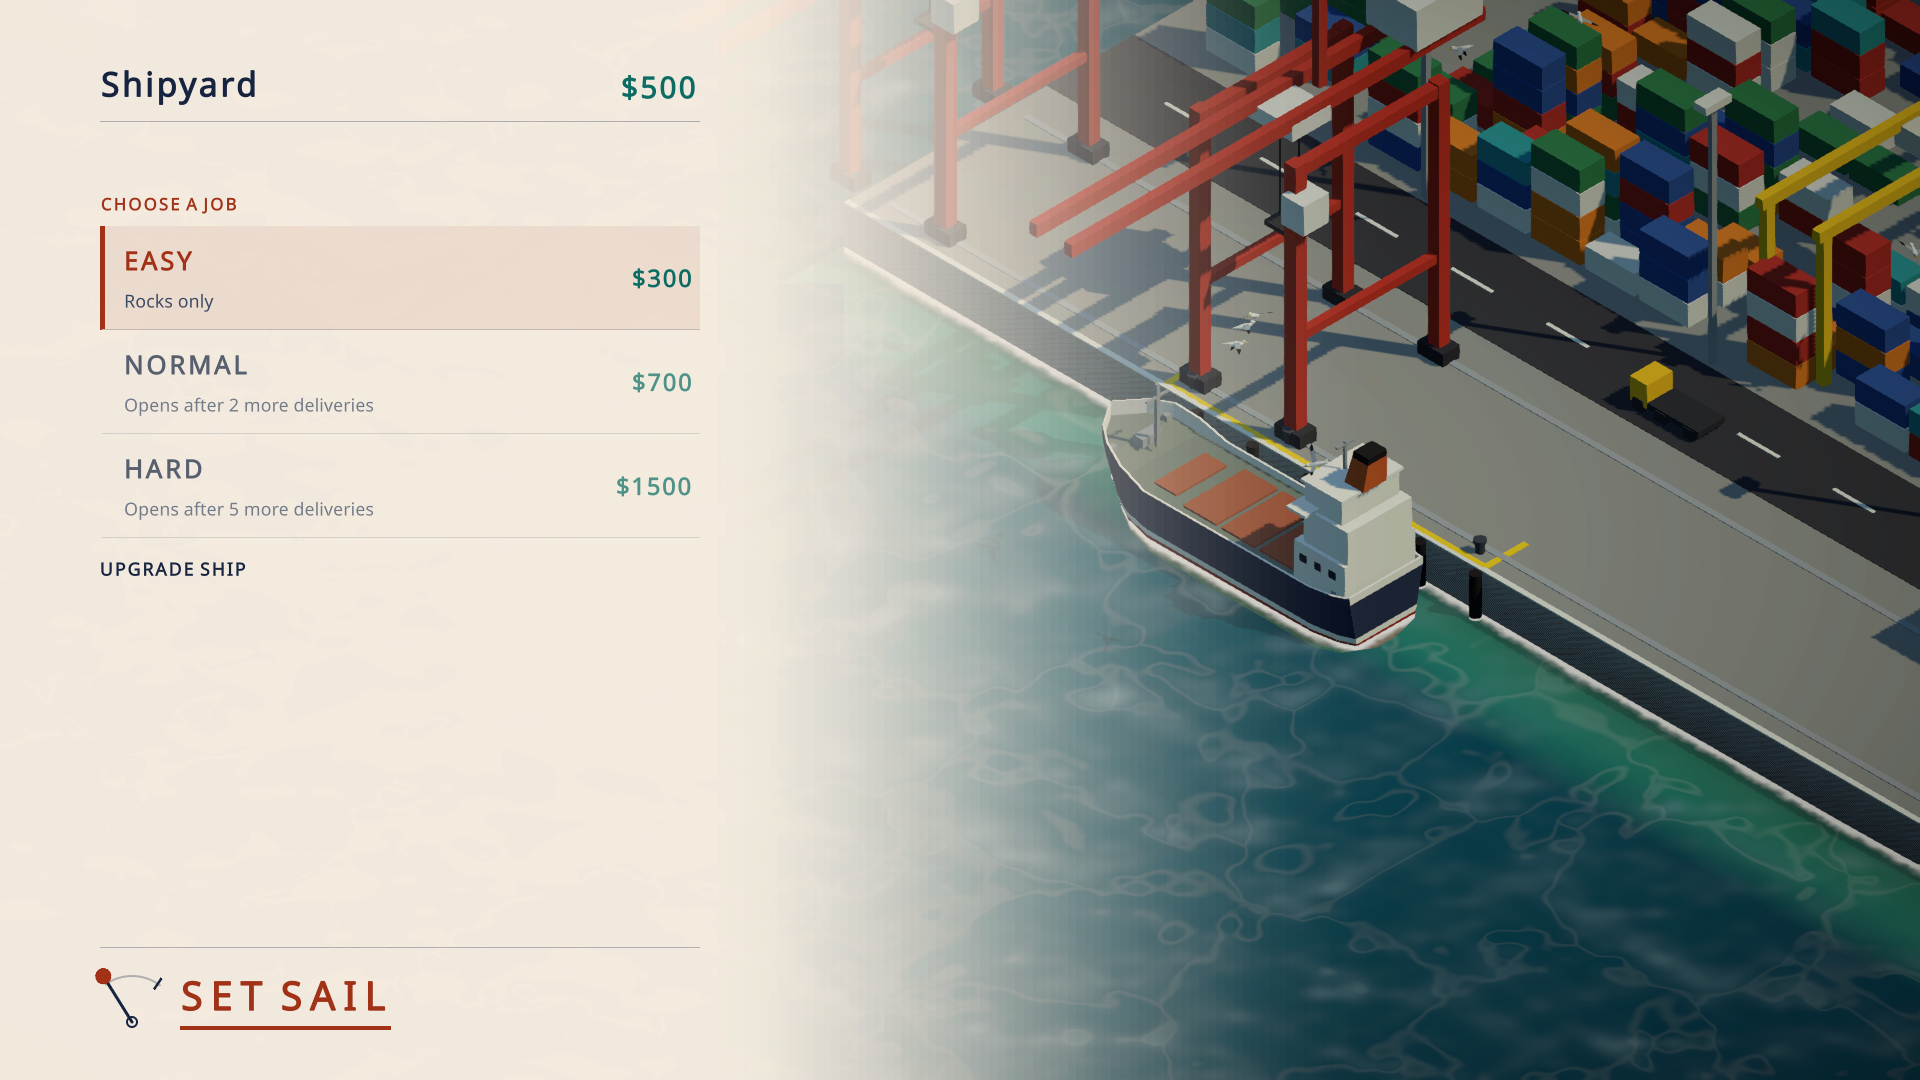
\includegraphics[width=0.8\textwidth]{Document/GameDev/images/Shipyard.png}
\caption{หน้าจออู่ต่อเรือ (UI-03)}
\label{fig:ui_shipyard}
\end{figure}

จากภาพที่ \ref{fig:ui_shipyard} ด้านซ้ายแสดงยอดเงินและรายการงานขนส่ง 3 ระดับ พร้อมค่าตอบแทนและเงื่อนไขการปลดล็อก ส่วนปุ่มอัปเกรดเรือเปิดรายการอัปเกรด 5 ด้าน ได้แก่ เครื่องยนต์ หางเสือ ยามระวังหน้า ตัวเรือ และลูกเรือ ซึ่งต้องใช้ทั้งเงินและใบรับรองทักษะภาษาที่ได้จากการใช้รูปประโยคมาตรฐาน และปุ่ม SET SAIL เริ่มการเดินเรือ ด้านขวาแสดงเรือของผู้เล่นที่ท่าเรือ

\subsubsection{UI-04: หน้าจอสรุปผล (Result Screen)}

หน้าจอสรุปผลแสดงหลังจบการเดินเรือทุกรอบ ดังภาพที่ \ref{fig:ui_result}

\begin{figure}[!htbp]
\centering
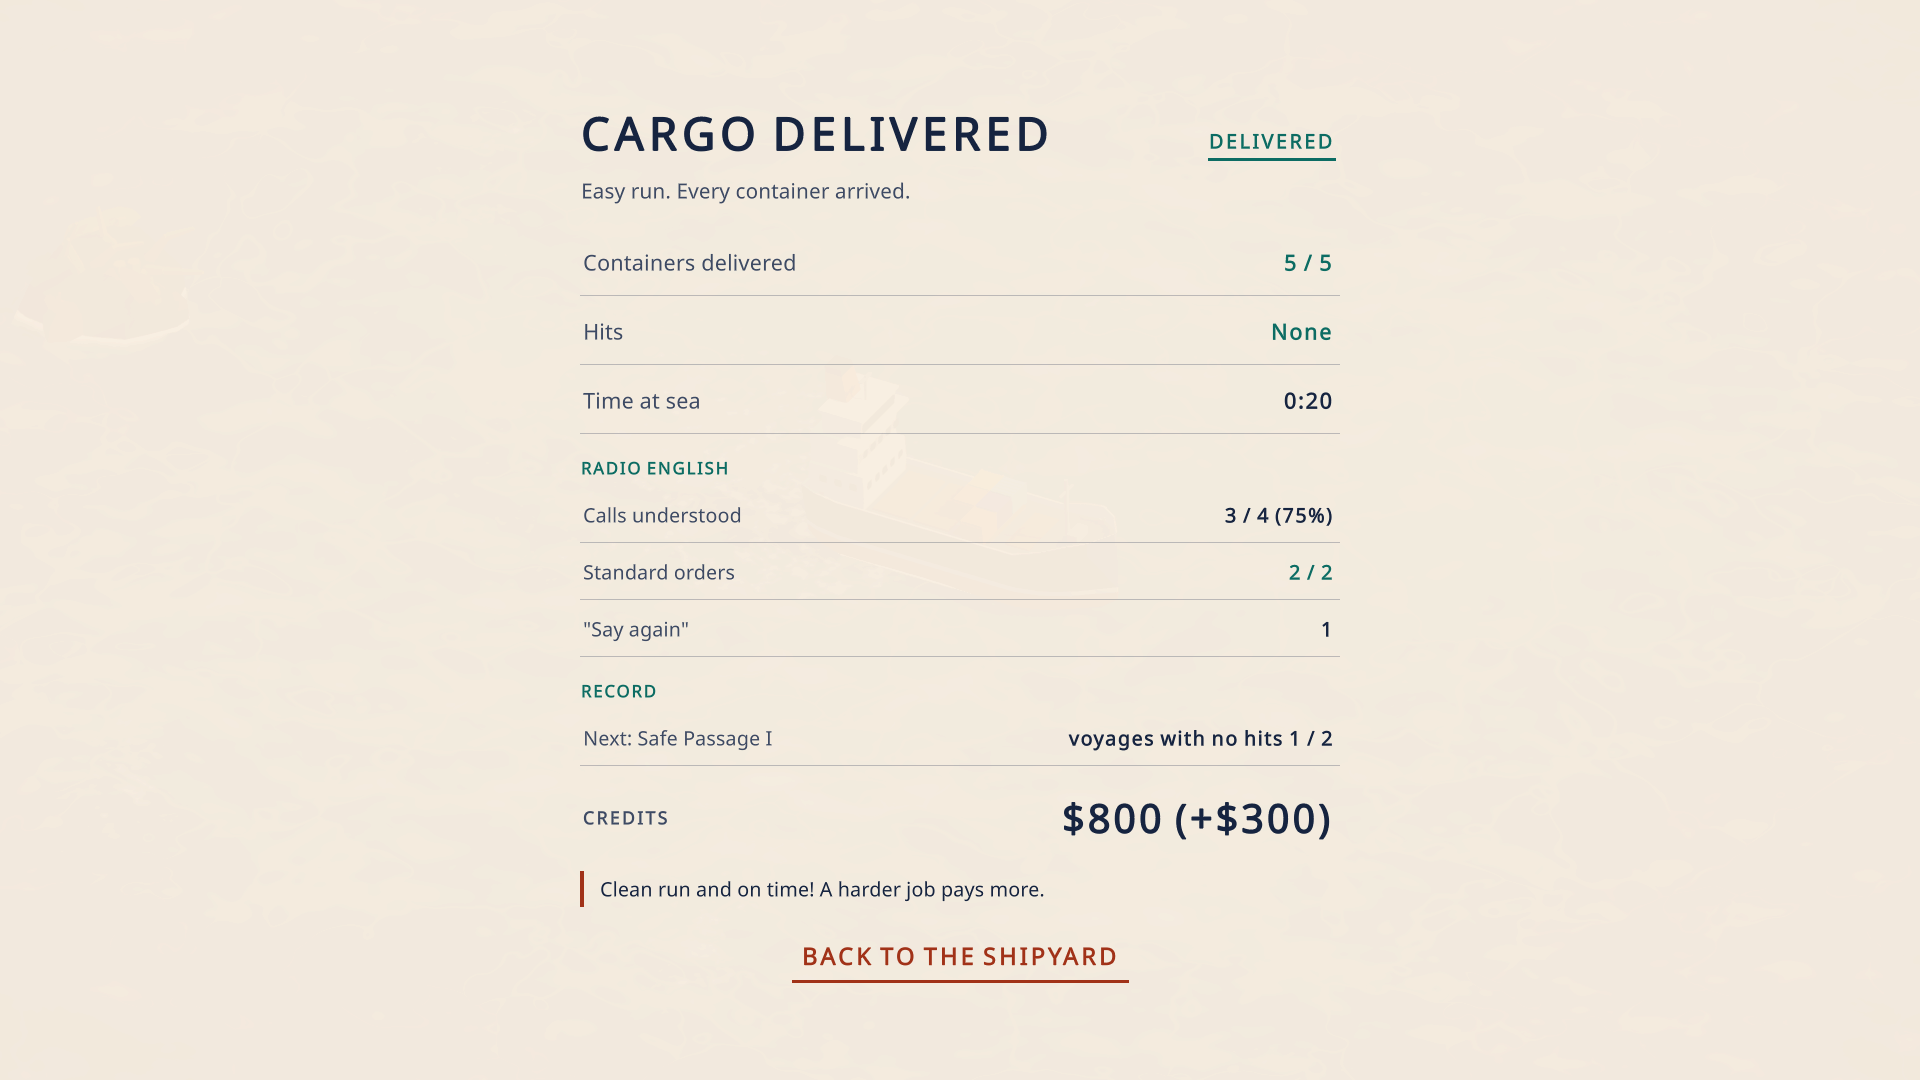
\includegraphics[width=0.8\textwidth]{Document/GameDev/images/Victory.png}
\caption{หน้าจอสรุปผล (UI-04)}
\label{fig:ui_result}
\end{figure}

จากภาพที่ \ref{fig:ui_result} หัวข้อแสดง CARGO DELIVERED (หรือ MISSION COMPLETE ในโหมดเนื้อเรื่อง) ส่วนบนแสดงผลการเดินเรือ ได้แก่ จำนวนตู้สินค้าที่ส่งถึง จำนวนครั้งที่ชน และเวลาที่ใช้ ส่วน RADIO ENGLISH สรุปการสื่อสาร ได้แก่ สัดส่วนคำสั่งที่ลูกเรือเข้าใจ จำนวนคำสั่งมาตรฐาน จำนวนครั้งที่ลูกเรือขอให้พูดซ้ำ เวลาเฉลี่ยในการสั่งหลังได้รับคำเตือน และจำนวนคำสั่งฉุกเฉินที่ทันเวลา โดยแต่ละบรรทัดแสดงเมื่อมีข้อมูลในรอบนั้น ส่วน RECORD แสดงความคืบหน้าของใบรับรองถัดไป และด้านล่างแสดงเงินที่ได้รับพร้อมคำแนะนำสำหรับรอบถัดไป หากเรืออับปาง หัวข้อจะเปลี่ยนเป็น SHIP LOST และแสดงจำนวนตู้สินค้าที่เสียและค่าลากเรือกลับท่าแทนจำนวนตู้สินค้าที่ส่งถึง

\subsubsection{UI-05: เมนูหยุดเกม (Pause)}

เมื่อกดปุ่ม PAUSE หรือ Esc ระหว่างเดินเรือ เกมจะหยุดและแสดงเมนูหยุดเกมทับหน้าจอเล่นเกม ดังภาพที่ \ref{fig:ui_pause}

\begin{figure}[!htbp]
\centering
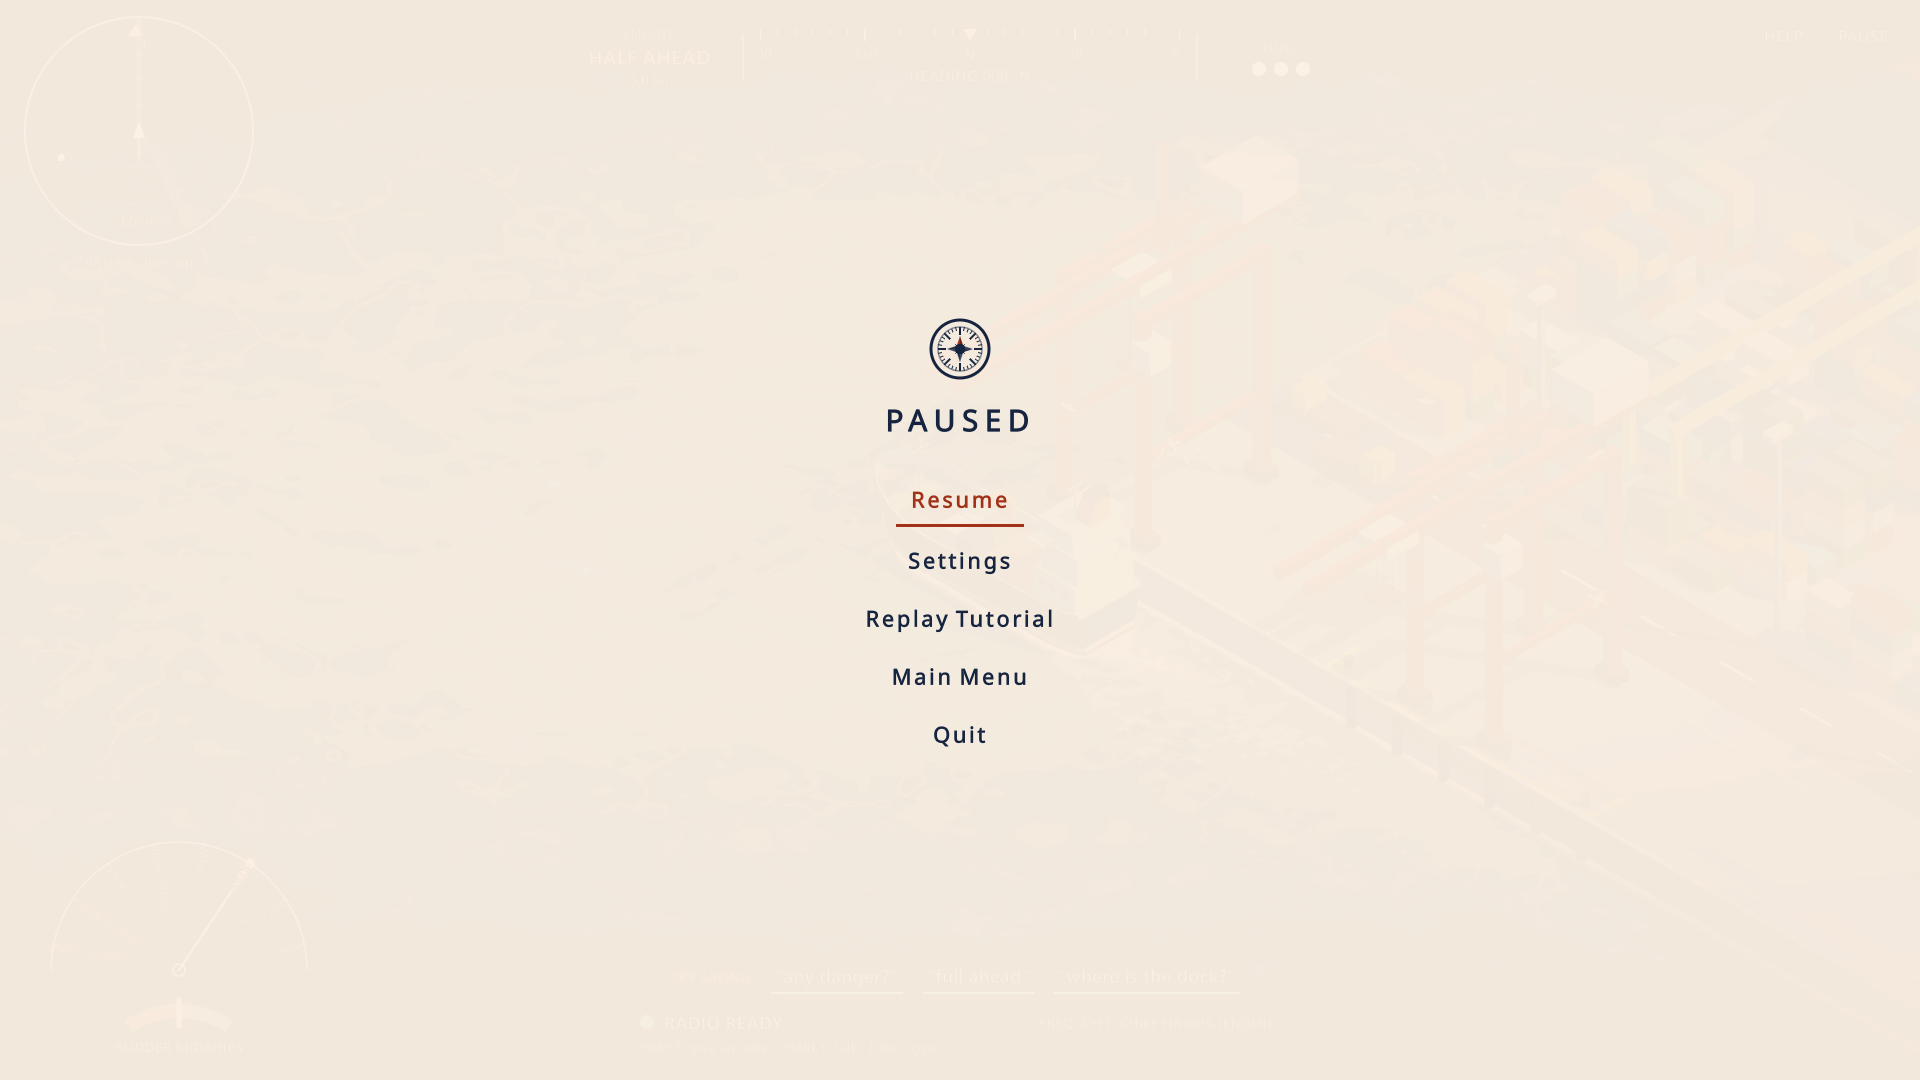
\includegraphics[width=0.8\textwidth]{Document/GameDev/images/Pause.png}
\caption{เมนูหยุดเกม (UI-05)}
\label{fig:ui_pause}
\end{figure}

จากภาพที่ \ref{fig:ui_pause} เมนูหยุดเกมประกอบด้วย Resume Settings Replay Tutorial Main Menu และ Quit และเกมยกเลิกการบันทึกเสียงที่ค้างอยู่เมื่อหยุดเกม

\subsubsection{UI-06: หน้าจอตั้งค่า (Settings)}

หน้าจอตั้งค่าเปิดได้ทั้งจากหน้าจอหลักและเมนูหยุดเกม ดังภาพที่ \ref{fig:ui_settings}

\begin{figure}[!htbp]
\centering
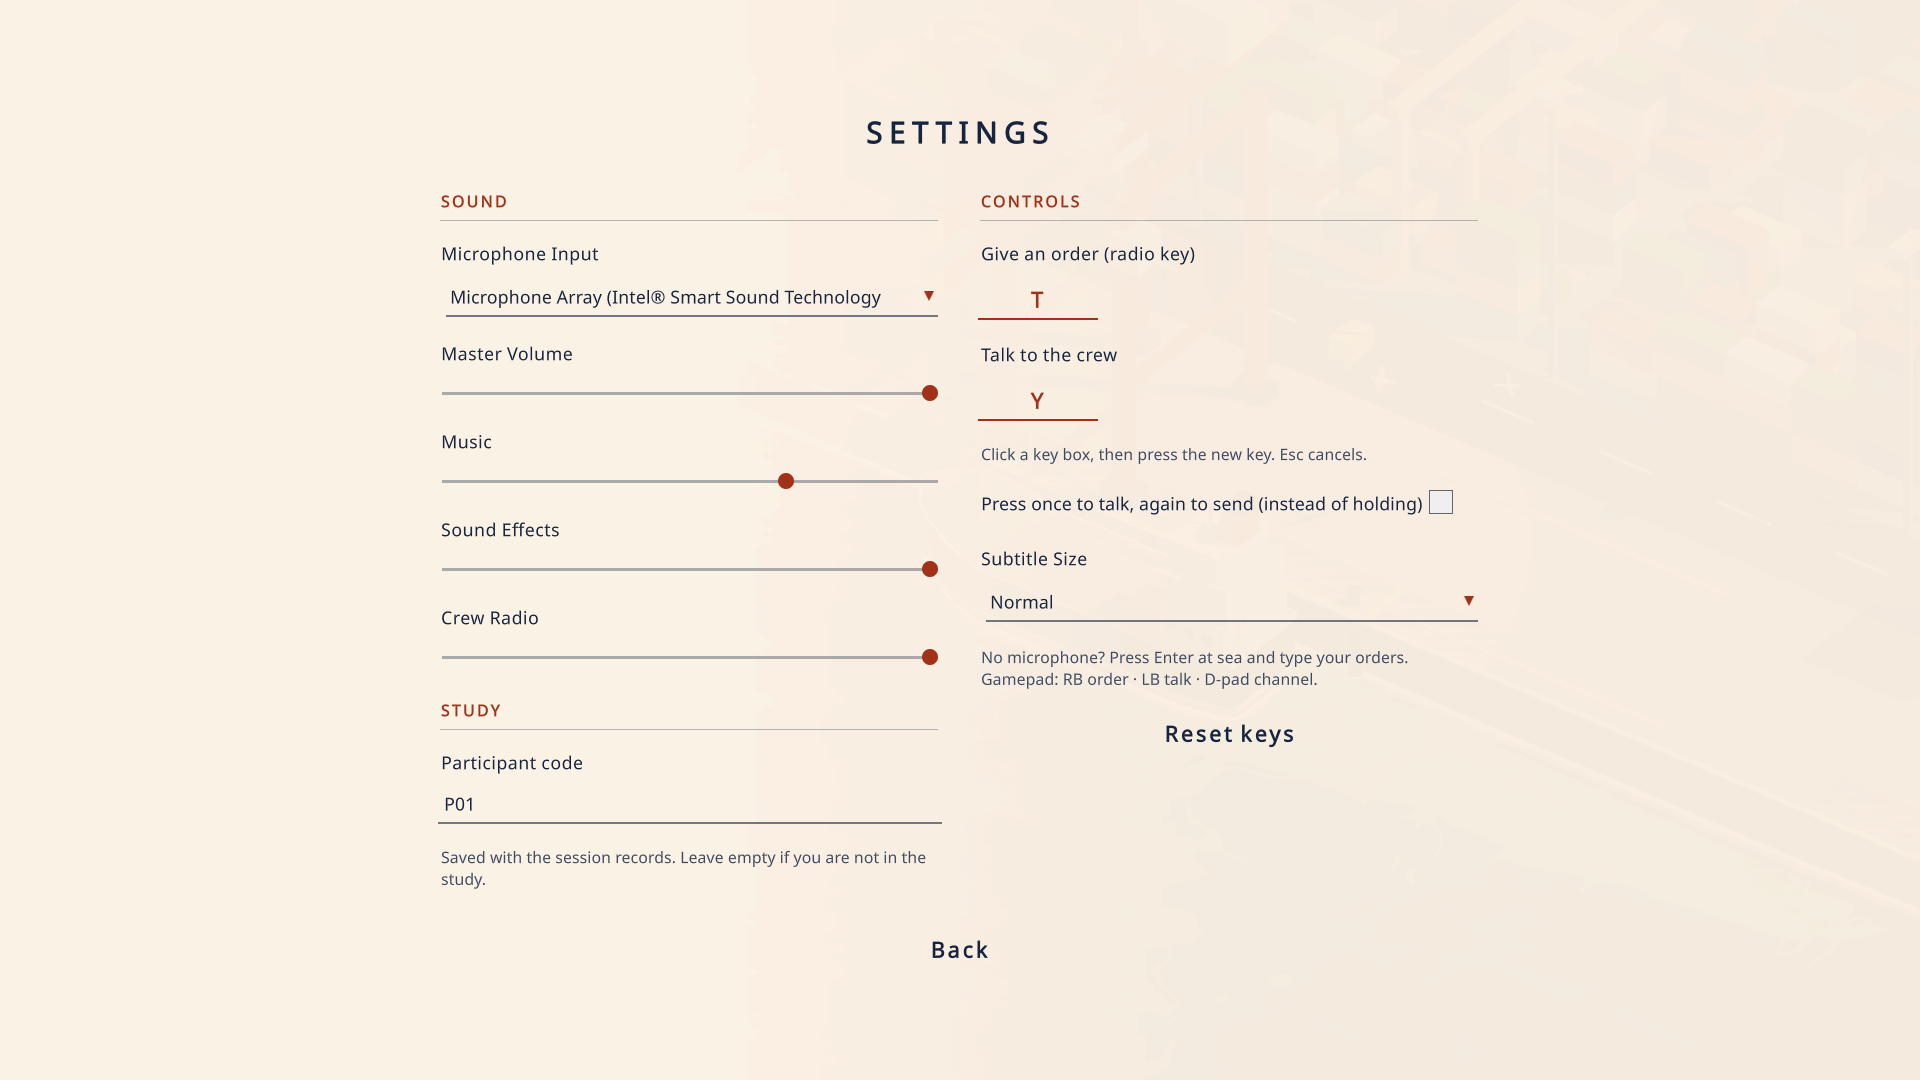
\includegraphics[width=0.8\textwidth]{Document/GameDev/images/Settings.png}
\caption{หน้าจอตั้งค่า (UI-06)}
\label{fig:ui_settings}
\end{figure}

จากภาพที่ \ref{fig:ui_settings} หน้าจอตั้งค่าแบ่งเป็น 3 ส่วน ได้แก่ SOUND (เลือกไมโครโฟน ระดับเสียงรวม ดนตรี เสียงประกอบ และเสียงวิทยุของลูกเรือ) CONTROLS (ปุ่มสั่งการ ปุ่มสนทนา โหมดกดครั้งเดียวเพื่อพูดและกดอีกครั้งเพื่อส่งแทนการกดค้าง และขนาดคำบรรยาย พร้อมคำแนะนำการพิมพ์คำสั่งและการใช้จอยเกม) และ STUDY (รหัสผู้เข้าร่วม ซึ่งบันทึกไปพร้อมกับแฟ้มบันทึกผล และเว้นว่างได้หากไม่ได้เข้าร่วมการทดลอง)
